\clearpage
\section{Hector SLAM}
During development we decided to use hector slam to make a 2D SLAM map. Hector mapping is a ROS library that we can use without odomety. %http://wiki.ros.org/hector_mapping
We could then skip using the optical flow sensor for publishing movement on a x and y scale. Hector mapping uses reference points in its surroundings to make keep track of movement in a x and y scale. You can also give hector mapping information about movement in z scale, tilt and yaw. That is a big benefit for a robot that is going over big changes in terrain or even flying. 

Hector mapping need laser input published over the laser scan node, and also tf (transform) information about the robot. The tf represents difference in height of a laser from the ground or a offset in x,y and z coordinates. A robotic arm with multiple joints would have a transform on each of them so the system could calculate movement of the sensor located on the arm.

\begin{figure}[H]
	\centering
	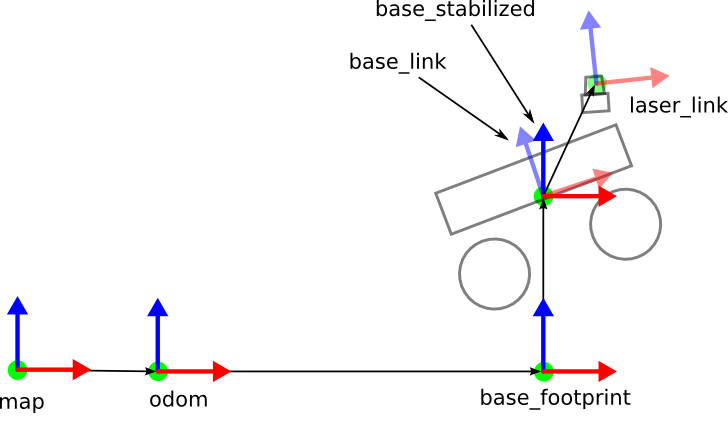
\includegraphics[width=.3\linewidth]{images/tf.png}
	\caption{transform of robot points.} %http://wiki.ros.org/hector_slam/Tutorials/SettingUpForYourRobot
\end{figure}

We took a single measurement using the laser and hector SLAM and got this picture of group room H101 in Aalborg University Esbjerg and compared it to the floor plan. 

\begin{figure}[H]
	\centering
	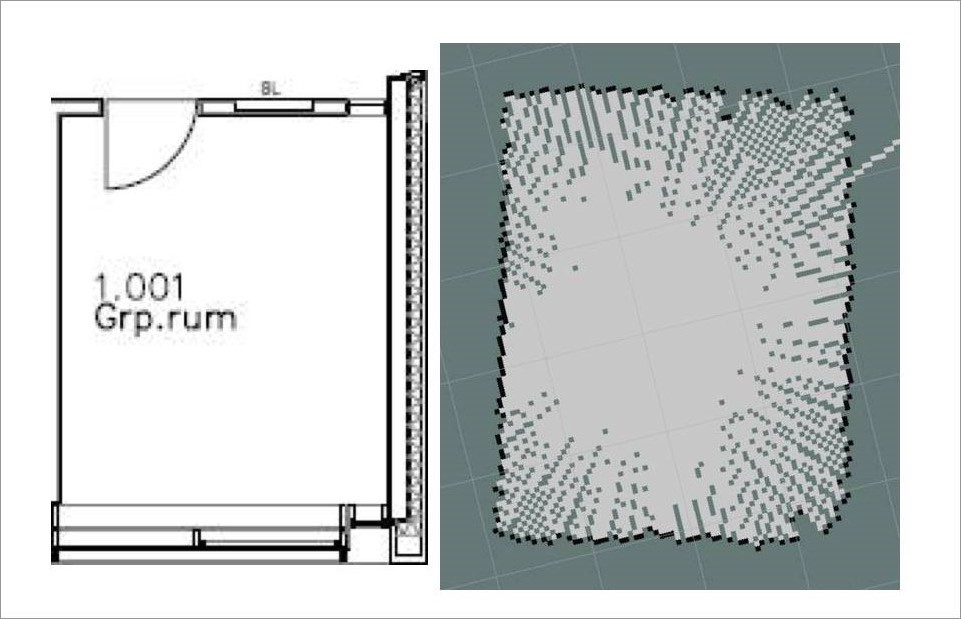
\includegraphics[width=.3\linewidth]{images/compare.jpg}
	\caption{Room H101 Aalborg University Esbjerg.}
\end{figure}

The hector map picture is a screen shot taken from rviz. Rviz is a visualization tools included in ROS to see laser measurements and 2D map in the making. %http://wiki.ros.org/rviz

\begin{figure}[H]
	\centering
	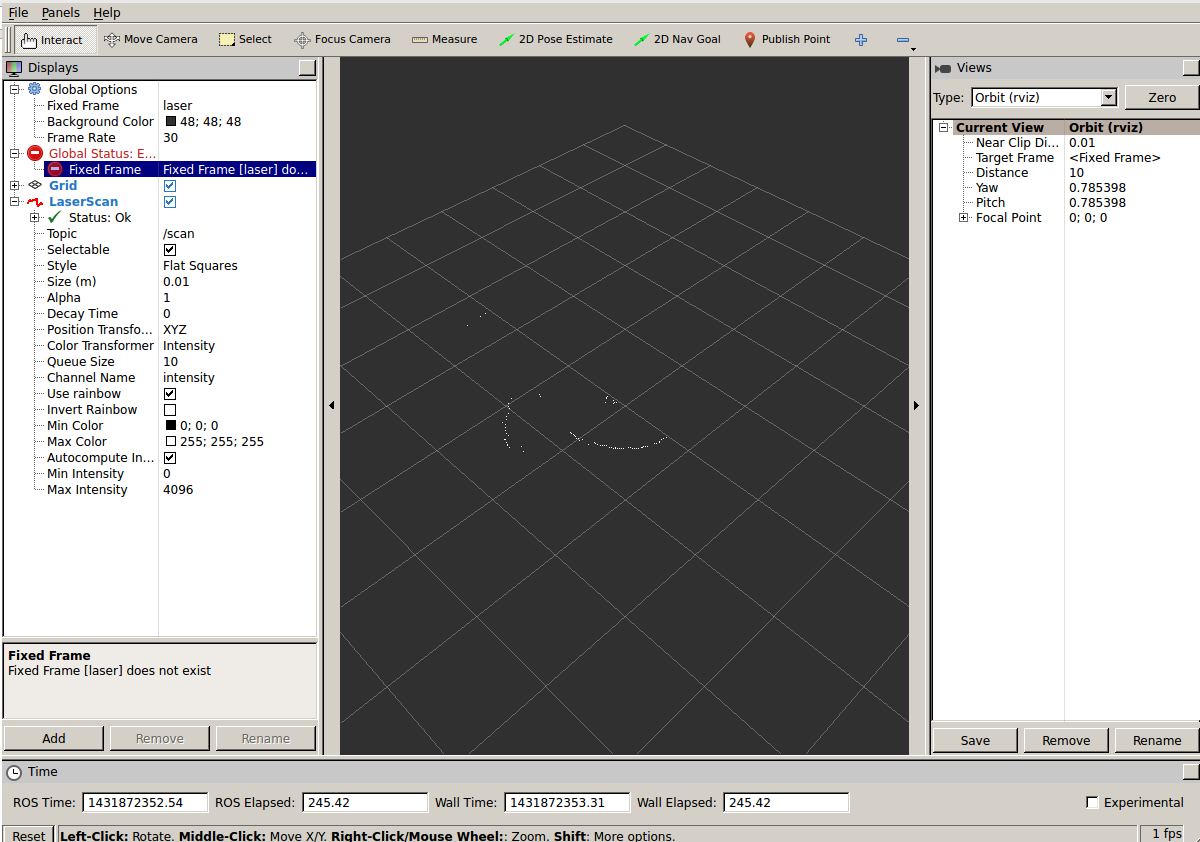
\includegraphics[width=.3\linewidth]{images/rviz.png}
	\caption{Rviz visualization tools package in ROS.}
\end{figure}

Hector mapping takes the information given from the transform and laser measurement and makes a 2D map from it. Here is a small flowchart explaining the steps.

\begin{figure}[H]
	\centering
	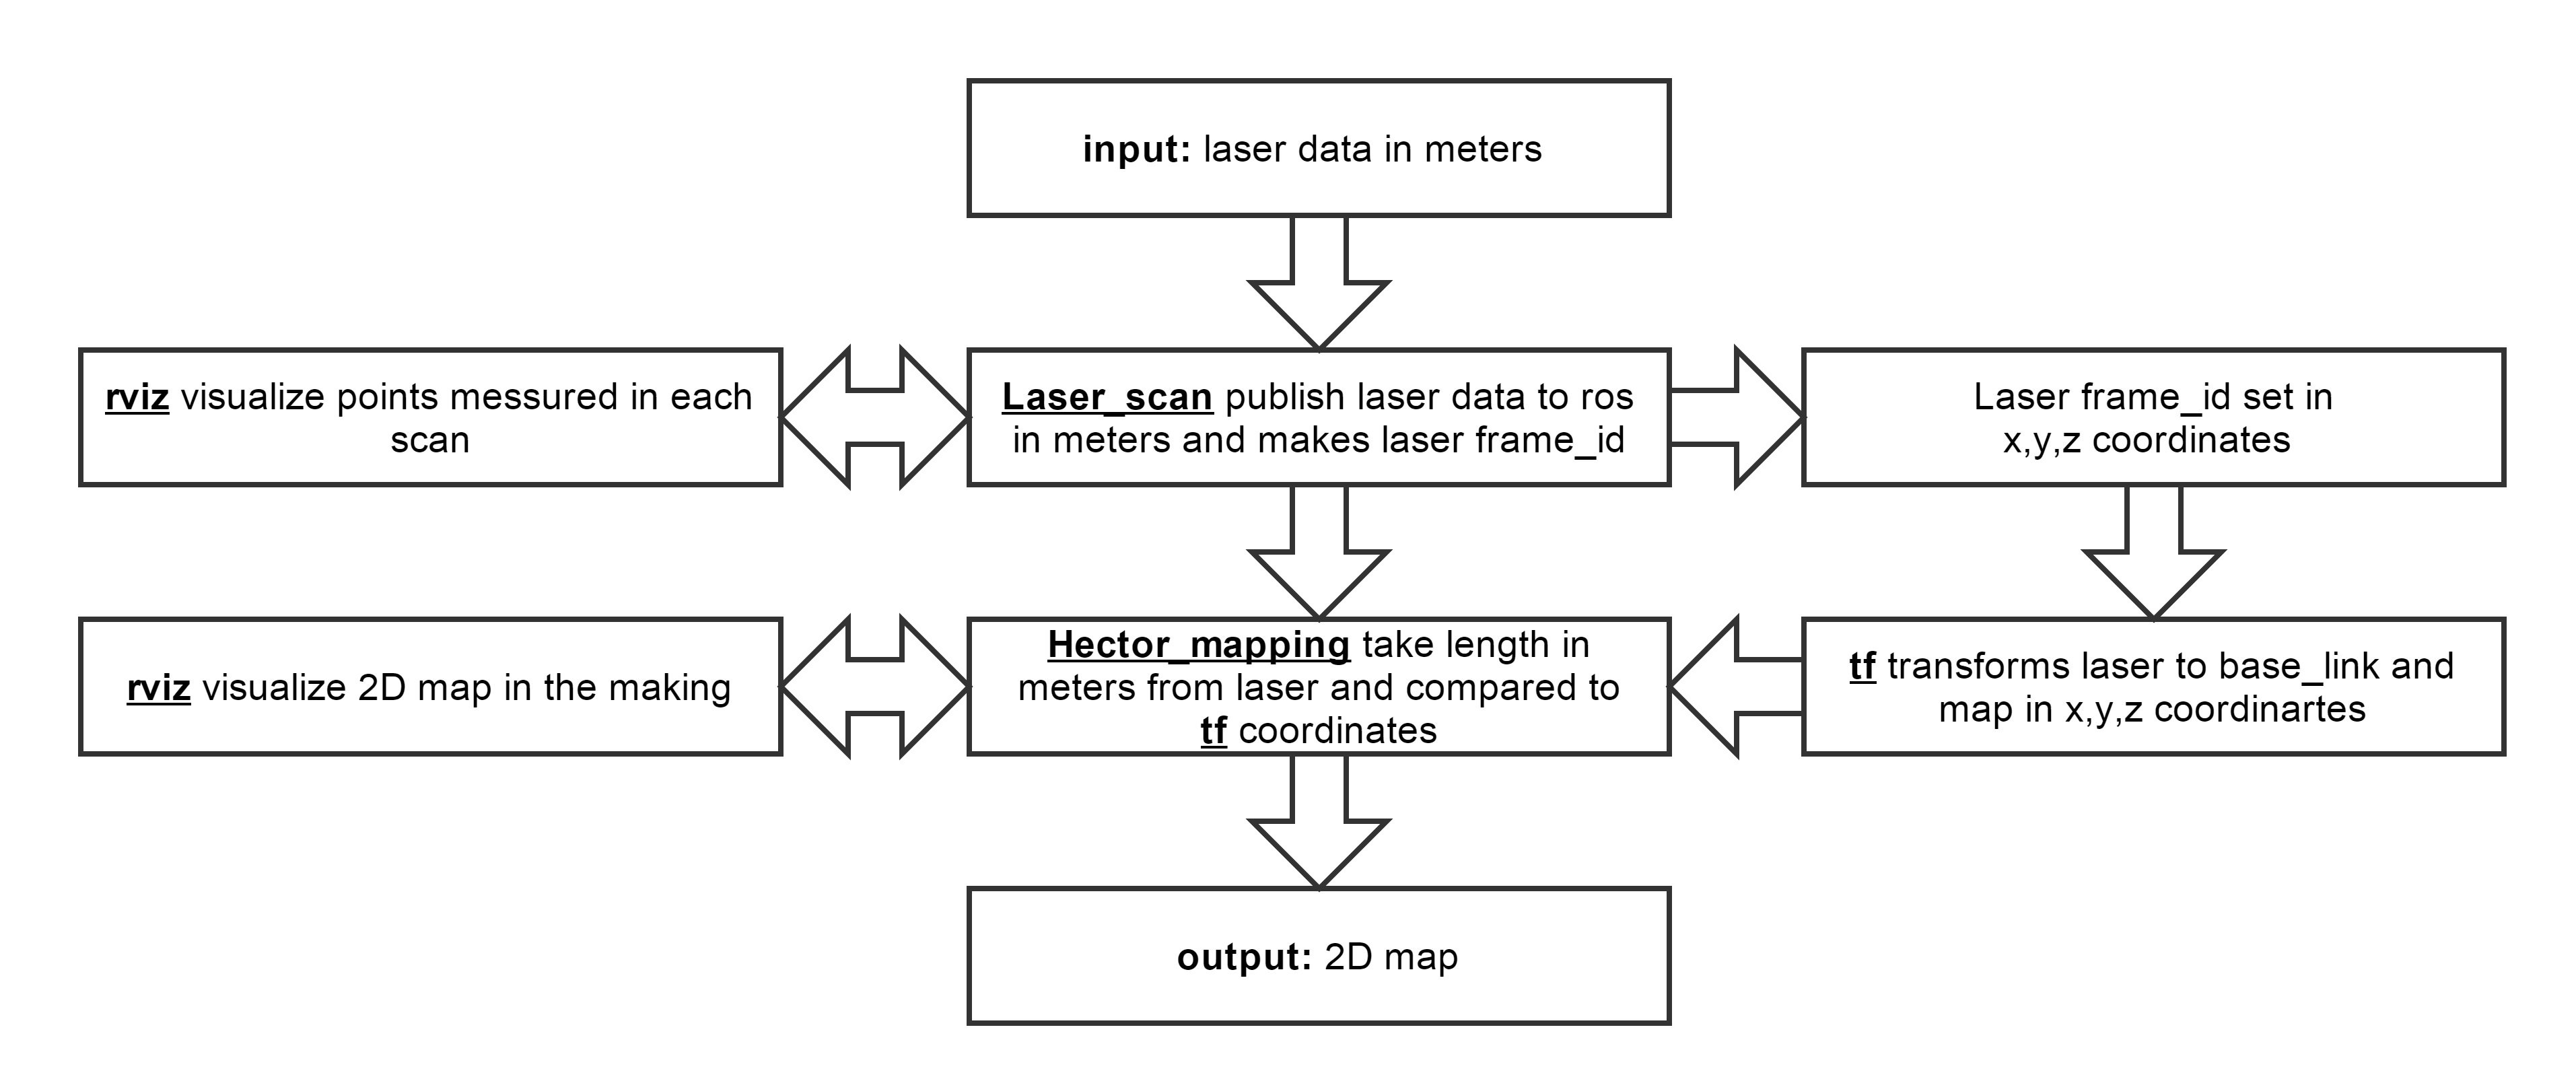
\includegraphics[width=.3\linewidth]{images/hector_flow.png}
	\caption{Hector mapping flowchart.}
\end{figure}

